%\documentclass[10pt]{article}
%\usepackage{tikz}
%\usetikzlibrary{calc}
%\begin{document}
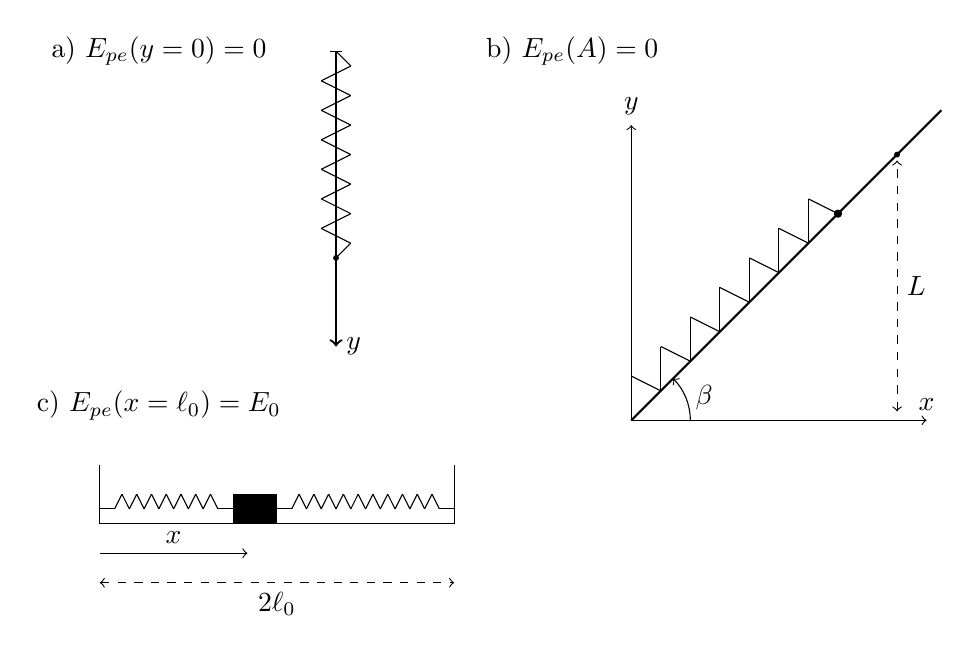
\begin{tikzpicture}[scale=.75]

\draw (-6,0) node{a) $E_{pe}(y=0)=0$};
\draw[thick,->] (-3,0) -- (-3,-5) node[right]{$y$};
\draw (-3.1,0) -- (-2.9,0) node[right]{$\ptO$};
\draw (-3,0) -- (-2.75,-.25);
\foreach \x in {.5,1,...,3}
{\draw (-2.75,-\x+.25) -- (-3.25,-\x);
\draw (-3.25,-\x) -- (-2.75,-\x-.25);}
\draw (-2.75,-3.25) -- (-3,-3.5);
\fill (-3,-3.5) circle(.05) node[right]{$\ptM$};

\draw (1,0) node{b) $E_{pe}(A)=0$};
\foreach \x in {0,.5,...,2.5}
{\draw (2+\x,-5.5+\x) -- (2+\x+.5,-5.5+\x-.25);
\draw (2+\x+.5,-5.5+\x-.25) -- (2+\x+.5,-5.5+\x+.5);}
\draw (5,-2.5) -- (5.5,-2.75);
\draw[thick] (2,-6.25) -- (7.25,-1);
\draw[->] (2,-6.25) -- (7,-6.25) node[above]{$x$};
\draw[->] (2,-6.25) -- (2,-1.25) node[above]{$y$};
\draw[<->,dashed] (6.5,-6.1) -- (6.5,-1.85) node[right,midway]{$L$};
\fill (6.5,-1.75) circle(.05) node[above]{$\ptA$};
\draw[->] (3,-6.25) arc(0:45:1) node[midway,right]{$\beta$};
\fill (5.5,-2.75) circle(.07) node[below]{$\ptM$};
\draw (2,-6.25) node[below]{$\ptO$};

\draw (-6,-6) node{c) $E_{pe}(x=\ell_0)=E_0$};

\draw (-7,-7) -- (-7,-8) -- (-1,-8) -- (-1,-7);
\draw (-7,-7.75) -- (-6.75,-7.75);
\foreach \x in {0,.25,...,1.5}
{\draw (-6.75+\x,-7.75) -- (-6.625+\x,-7.5);
\draw (-6.625+\x,-7.5) -- (-6.5+\x,-7.75);}
\draw (-1,-7.75) -- (-1.25,-7.75);
\foreach \x in {3,3.25,...,5.25}
{\draw (-6.75+\x,-7.75) -- (-6.625+\x,-7.5);
\draw (-6.625+\x,-7.5) -- (-6.5+\x,-7.75);}
\fill (-4.75,-8) rectangle (-4,-7.5);
\draw (-5,-7.75) -- (-4.75,-7.75);
\draw (-4,-7.75) -- (-3.75,-7.75);
\draw[dashed,<->] (-7,-9) -- (-1,-9) node[below,midway]{$2\ell_0$};
\draw[->] (-7,-8.5) -- (-4.5,-8.5) node[midway,above]{$x$};



\end{tikzpicture}

%\end{document}
